\section{Spectral Behaviour of LPS Graphs}
  \label{sec:spectral}

  \subsection{Algebraic connectivity along the relaxation trajectory}
    \label{sec:spectral:lambda2}

    Fix $p$ and let $q \to \infty$.
    From~\eqref{eq:ramanujan-laplacian} and the Alon--Boppana
    bound~\cite{Alon1986},
    \begin{equation}
      \label{eq:lambda2-limit}
      \lambda_2(n) \;\longrightarrow\; \lambda_2^*(p)
      \;:=\; 1 - \frac{2\sqrt{p}}{p+1} \;>\; 0.
    \end{equation}

    \begin{proposition}[Asymptotic constancy of $\Lambda_{\mathrm{proj}}$]
      \label{prop:Lambda-constant}
      Under Hypotheses~\ref{hyp:closure} and~\ref{hyp:saturation}, for the LPS
      family at fixed $p$,
      \begin{equation}
        \label{eq:Lambda-constant}
        \Lambda_{\mathrm{proj}}(n) \;\longrightarrow\; \Lambda_0(p)
        \;:=\; \frac{C\,\lambda_2^*(p)}{A_{\min}^2}
        \qquad \text{as } n \to \infty.
      \end{equation}
    \end{proposition}

    \noindent
    Proposition~\ref{prop:Lambda-constant} shows that the admissibility threshold
    is asymptotically static in this model.
    The dynamical variable driving stabilisation is therefore the saturation
    condition $N(\lambda_i; n) \geq k\,\dim\rho_{\lambda_i}$, not the variation
    of $\Lambda_{\mathrm{proj}}$.

  \subsection{Kesten--McKay spectral density}
    \label{sec:spectral:kesten}

    As $q \to \infty$ with $p$ fixed, the empirical spectral measure of
    $L_{X^{p,q}}$ converges weakly to the \emph{Kesten--McKay
measure}~\cite{McKay1981,Kesten1959}
    \begin{equation}
      \label{eq:kesten-mckay}
      \mathrm{d}\mu_{\mathrm{KM}}^{(p)}(\lambda)
      \;=\; \rho_{\mathrm{KM}}^{(p)}(\lambda)\,\mathrm{d}\lambda,
      \qquad
      \rho_{\mathrm{KM}}^{(p)}(\lambda)
      \;=\; \frac{(p+1)\sqrt{4p - (p+1)^2(1-\lambda)^2}}
      {2\pi\,p\,\bigl(1 - (1-\lambda)^2\bigr)},
    \end{equation}
    supported on $[\lambda_-, \lambda_+]$ with
    $\lambda_\pm = 1 \mp 2\sqrt{p}/(p+1)$.
    The density is symmetric about $\lambda = 1$:
    $\rho_{\mathrm{KM}}(\lambda) = \rho_{\mathrm{KM}}(2 - \lambda)$.

    \begin{figure}[h]
      \centering
      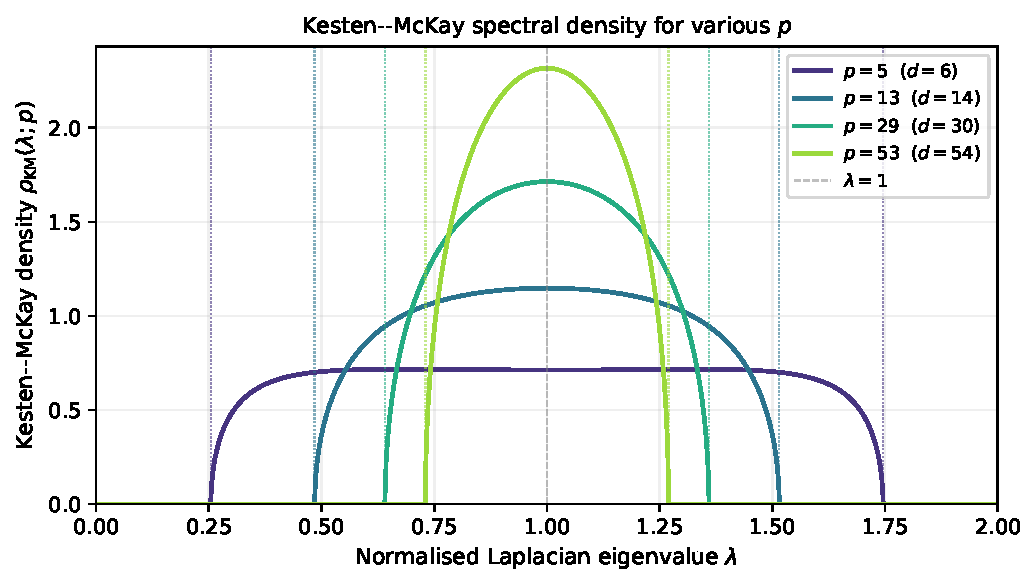
\includegraphics[width=0.82\textwidth]{fig1_km_density}
      \caption{Kesten--McKay spectral density $\rho_{\mathrm{KM}}^{(p)}(\lambda)$
        for $(p+1)$-regular graphs with $p \in \{5, 13, 29, 53\}$.
        The support $[\lambda_-, \lambda_+]$ narrows as $p$ grows.
        Dashed vertical lines mark the three normalised eigenvalue levels of
        the $2I$ ord-5 ADE case ($\lambda_1 = 20/24$, $\lambda_2 = 1$,
        $\lambda_3 = 30/24$).
        All three levels lie inside the support for $p \leq 53$; the structural
        identity $F_{\mathrm{KM}}(1) = 1/2$ follows from the symmetry of the
        density about $\lambda = 1$.}
      \label{fig:km-density}
    \end{figure}

    \begin{remark}[Relation to the $S^3$ spectral measure]
  As $p \to \infty$, the Kesten--McKay measure converges to the spectral
  measure of the $S^3$ Laplacian~\cite{Beau2026a1}.
  The LPS family therefore interpolates between the discrete Ramanujan regime
  and the $S^3$ continuum.
    \end{remark}

  \subsection{Monotonicity and linear growth of the spectral counting function}
    \label{sec:spectral:counting}

    Write $F_{\mathrm{KM}}(\lambda) := \mu_{\mathrm{KM}}^{(p)}((-\infty, \lambda])$
    for the cumulative distribution function.
    By weak convergence and the identification~\eqref{eq:index-id}:
    \begin{equation}
      \label{eq:counting-linear}
      N(\lambda;\, n) \;\sim\; F_{\mathrm{KM}}(\lambda)\cdot n
      \qquad (n \to \infty).
    \end{equation}

    \begin{lemma}[Monotonicity]
      \label{lem:monotonicity}
      For $\lambda$ in the interior of $[\lambda_-, \lambda_+]$, $N(\lambda; n)$
      is strictly increasing in $n$ for all sufficiently large $n$.
    \end{lemma}

    \begin{proof}
      Since $F_{\mathrm{KM}}(\lambda) > 0$ for $\lambda$ in the interior of the
      support and $|V(G(n))| \sim n$ is strictly increasing,
      $N(\lambda;n) \sim F_{\mathrm{KM}}(\lambda)\cdot n$ is strictly increasing.
    \end{proof}

    \begin{proposition}[Linear growth of projectable mode count]
      \label{prop:Nproj-linear}
      For the LPS family at fixed $p$ and $\lambda \leq \Lambda_0(p)$,
      \begin{equation}
        \label{eq:Nproj-linear}
        N(\lambda;\, n) \;\sim\; F_{\mathrm{KM}}(\lambda)\cdot n
        \qquad \text{as } n \to \infty.
      \end{equation}
    \end{proposition}

    \noindent
    For the three ADE eigenvalue levels $\lambda_1 < \lambda_2 < \lambda_3$
    of~\cite{Beau2026a4}, define
    \begin{equation}
      \label{eq:KM-coefficients}
      c_i(p) \;:=\; F_{\mathrm{KM}}(\lambda_i)
      \;=\; \int_{\lambda_-}^{\lambda_i} \rho_{\mathrm{KM}}^{(p)}(x)\,\mathrm{d}x,
      \qquad i = 1,2,3,
    \end{equation}
    satisfying $0 < c_1(p) < c_2(p) < c_3(p) \leq 1$.
    Since $\lambda_2^{\mathrm{norm}} = 1$ for all three-level ADE cases and
    $F_{\mathrm{KM}}(1) = 1/2$ by symmetry of the Kesten--McKay density,
    \begin{equation}
      \label{eq:c2-universal}
      c_2(p) \;=\; \tfrac{1}{2}
      \qquad \text{for all } p.
    \end{equation}
    This is a structural identity, not a numerical coincidence.

  \subsection{Stabilisation ranks and mass formula}
    \label{sec:spectral:stabilisation}

    By Lemma~\ref{lem:monotonicity}, Definition~\ref{def:nproj} is well-posed.
    Inverting Proposition~\ref{prop:Nproj-linear}:
    \begin{equation}
      \label{eq:nproj-value}
      n_{\mathrm{proj}}(\lambda_i)
      \;\sim\; \frac{k\,\dim\rho_{\lambda_i}}{c_i(p)}.
    \end{equation}
    The effective stabilisation mass and inter-generation mass ratio are therefore
    \begin{equation}
      \label{eq:mass-formula}
      \mathcal{M}_i
      \;\sim\; \frac{c_i(p)\,E_{\mathrm{P}}}{k\,\dim\rho_{\lambda_i}},
      \qquad
      \frac{\mathcal{M}_i}{\mathcal{M}_j}
      \;=\; \frac{c_i(p)}{c_j(p)}\cdot
      \frac{\dim\rho_{\lambda_j}}{\dim\rho_{\lambda_i}}.
    \end{equation}
    The universal constant $k$ cancels in all ratios.
    The first factor $c_i/c_j$ is determined by the spectral geometry of the LPS
    substrate; the second factor $\dim\rho_j/\dim\rho_i$ is determined by the
    representation theory of the ADE group.
    The two mechanisms are independent and act multiplicatively.
